\documentclass[12pt,twocolumn]{article}
\usepackage{fullpage}
\usepackage{amsmath}
\usepackage{graphicx}
\usepackage{enumerate}
\usepackage{float}
\usepackage{listings}
\usepackage{longtable}
\usepackage[table]{xcolor}
\usepackage{tabularx}
\usepackage{parskip}
\usepackage[round]{natbib}
\restylefloat{figure}
\title{Gamifying the Transcriptome}
\author{Chidube Ezeozue and Joel Brooks}

\begin{document}
\bibliographystyle{apalike}
\renewcommand\refname{Bibliography}
\maketitle

\begin{abstract}

\end{abstract}

\section*{Introduction}

\subsection*{Game Overview}
The game is designed to utilized human powered computation to explore transcriptome solutions for certain genes using experimental data from
RNA-seq. Experimental data is first mapped to a genome using a splicing aware read aligner such sat TopHat \citep{trapnell2009tophat}. From these mappings,
relative abidance levels of each exon within a gene are inferred.

When the user first starts the game, they are presented with a puzzle as shown in figure \ref{fig:game screen}. This puzzle represents
the relative abundance of exons within a gene. A player must clear all of the blocks in each column in order to complete the puzzle. Users accomplish this by 
creating and adding transcripts to their list. Single colored blocks represent the abundance of reads mapped just to that exon so they can be removed by any 
transcript that includes that exon. However, blocks with two colors represent the abundance of reads that were mapped to more than one exon. These ``linked"
blocks are removed when \emph{both} exons that the reads mapped to are selected, however, no exons can be selected in between the ``linked" blocks as
we assume a read can only map to more than one exon if those two exons appear contiguously within a transcript. Taking these rules into consideration, the user
tries to build a transcript list that removes all of the blocks in the puzzle and achieves a maximal score.

\begin{figure*}[h]

\centering
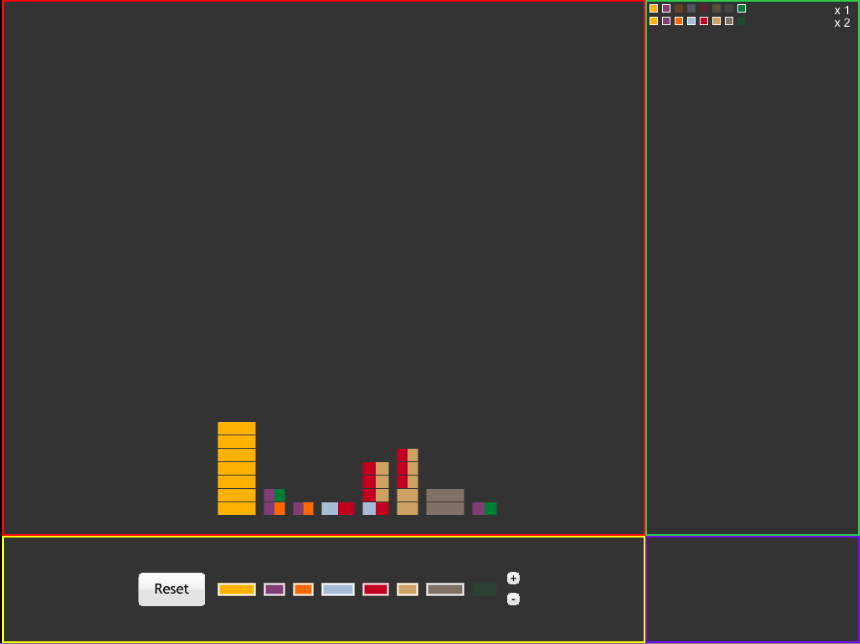
\includegraphics[width=6.5in]{gamescreen}
\caption{The main game interface}
\label{fig:gamescreen}
\end{figure*}

\section*{Methods}

\subsection*{Data acquisition and preparation}

\subsection*{Puzzle selection and construction}

\subsection*{Game implementation}
The game interface is built using the LimeJS HTML5 game framework. This framework provided methods for creating shapes,
animations, and handling user interaction events, allowing us to focus more on developing the core functionality of the game.
Additionally, the fact that the game is implemented in HTML5 and javascript means that it can be played natively in most 
popular browsers, as well as both desktop and mobile hardware.

We also made use of Kenneth Kelly's list of 22 colors of maximum contrast \citep{green2010colour}. This allowed us to assign a unique color each exon
in a particular puzzle that was easily distinguishable from the colors of all the other exons. This allowed us to present genes to 
users in a manner that was both visually appealing and functional.

\subsection*{Solution scoring}
How the user's will approach each puzzle is a function of both the given puzzle and how their solution for that puzzle is scored. Thus, we must have
a proper scoring system in order to influence user's to find accurate lists of transcripts for particular gene. However, as there is no real ``ground truth"
for a list of transcripts for a particular gene, we would like to have a scoring system that is independent of existing transcript annotations. Existing methods
for transcriptome assembly value small lists of unique transcripts, transcripts that include more exons, and transcripts that include more nucleotide bases (citations).
Thus we developed the following scoring metric for scoring transcript list $T$ :
\begin{equation*}
S(T) = d * \sum_{i=1}^{|T|} \log{|T_i|} * \sum_{j = 1}^{|T_i|} \log{n_{ik}}
\end{equation*}
\begin{equation*}
d = \frac{1}{1+e^{\gamma |T|}}
\end{equation*}
where $|T|$ is the number of transcripts in $T$, $|T_i|$ is the number of exons in transcript $T_i$, and $n_{ik}$ is the number of bases in exon $k$ of transcript $i$.
$d$ is a discount factor with parameter $\gamma$ that controls how longer lists of transcripts are devalued. Setting $\gamma = .001$ seemed to achieve the desired
discounting of long transcript lists within the context of the game. Furthermore, the $\log{|T_i|}$ factor ensures that transcripts that only contain one exon will not factor
into the player's score, which is a desirable property given that players often have to add transcripts with one exon in order to finish out a puzzle.

\section*{Results}

\subsection*{Gameplay statistics}

\subsection*{Player solutions}

\section*{Discussion}

\bibliography{frbib}

\end{document}
